\documentclass[a4paper,11pt, twocolumn]{article}
\usepackage[pdftex]{graphicx}
% \usepackage{amssymb}
\usepackage{amsmath}
\usepackage{epstopdf}
\usepackage[utf8]{inputenc}
\usepackage{titlesec}
% \usepackage[titletoc]{appendix}
% \titleformat{\chapter}[hang]{\bf\Huge}{\thechapter}{1cm}{}

\usepackage[colorlinks=true]{hyperref}
\hypersetup{urlcolor=blue,linkcolor=black,citecolor=black,colorlinks=true}
\bibliographystyle{plain}

\pagestyle{plain}
% -------------------- this stuff for code --------------------

\usepackage{anysize}
\marginsize{30mm}{30mm}{20mm}{20mm}

\newenvironment{formal}{%
  \def\FrameCommand{%
    \hspace{1pt}%
    {\color{blue}\vrule width 2pt}%
    {\color{formalshade}\vrule width 4pt}%
    \colorbox{formalshade}%
  }%
  \MakeFramed{\advance\hsize-\width\FrameRestore}%
  \noindent\hspace{-4.55pt}% disable indenting first paragraph
  \begin{adjustwidth}{}{7pt}%
  \vspace{2pt}\vspace{2pt}%
}
{%
  \vspace{2pt}\end{adjustwidth}\endMakeFramed%
}

\newenvironment{changemargin}[2]{\begin{list}{}{%
\setlength{\topsep}{0pt}%
\setlength{\leftmargin}{0pt}%
\setlength{\rightmargin}{0pt}%
\setlength{\listparindent}{\parindent}%
\setlength{\itemindent}{\parindent}%
\setlength{\parsep}{0pt plus 1pt}%
\addtolength{\leftmargin}{#1}%
\addtolength{\rightmargin}{#2}%
}\item }{\end{list}}

\usepackage{color}
\usepackage{dsfont}
\usepackage[bitstream-charter]{mathdesign}
\usepackage[scaled]{helvet}
\usepackage{inconsolata}


\definecolor{colKeys}{rgb}{0,0,0.9}
\definecolor{colIdentifier}{rgb}{0,0,0}
\definecolor{colString}{rgb}{0.7,0,0}
\definecolor{colComments}{rgb}{0,0.6,0}
\usepackage{listings}
\lstset{
  language=C++,
  stringstyle=\color{colString},
  keywordstyle=\color{colKeys},
  identifierstyle=\color{colIdentifier},
  commentstyle=\color{colComments},
  numbers=left,
  tabsize=4,
  frame=single,
  breaklines=true,
  basicstyle=\small\ttfamily,
  numberstyle=\tiny\ttfamily,
  framexleftmargin=0mm,
  xleftmargin=7mm,
  xrightmargin=7mm,
  frameround={tttt},
  captionpos=b
}

\usepackage{mathtools}
\usepackage{amsthm}
\newtheorem{definition}{Definition}
\newtheorem{theorem}{Theorem}
\DeclareMathOperator*{\argmin}{ArgMin\ }
\DeclareMathOperator*{\argmax}{ArgMax\ }

\usepackage[options]{algorithm}
\usepackage{algorithmic}

\usepackage[usenames,dvipsnames]{xcolor}
\makeatletter
\DeclareRobustCommand{\em}{%
  \@nomath\em \if b\expandafter\@car\f@series\@nil
  \normalfont \else \bfseries \fi}
\makeatother

%% Headers and footers
\usepackage{fancyhdr}
\usepackage[section]{placeins}
\pagestyle{fancy}
\fancyhf{}
\addtolength{\headwidth}{30pt}
\addtolength{\headwidth}{30pt}
\renewcommand{\headrulewidth}{0.4pt} % thickness of the header line
\renewcommand{\footrulewidth}{0.4pt} % thickness of the footer line
% \renewcommand{\chaptermark}[1]{\markboth{#1}{#1}} % chapter name
\renewcommand{\sectionmark}[1]{\markright{\thesection\ #1}}  % section name
\lhead[\fancyplain{}{\bf\thepage}]{\fancyplain{}{\bf\rightmark}} % display header
\rhead[\fancyplain{}{\bf\leftmark}]{\fancyplain{}{}} % display header
\fancyfoot[C]{\bf\thepage} % display footer (page number)
\fancyfoot[R]{\bf\today} % display footer (date)
\fancypagestyle{plain}{
	\fancyhead{} \renewcommand{\headrulewidth}{0pt}
}
% \newcommand{\clearemptydoublepage}{\newpage{\pagestyle{plain}\cleardoublepage}}

\usepackage[T1]{fontenc}
\usepackage{enumerate}
\usepackage{afterpage,lastpage,fancyhdr}
\usepackage[includeheadfoot,margin=2.5cm]{geometry}
\geometry{letterpaper}                   % ... or a4paper or a5paper or ...

% \DeclareGraphicsRule{.tif}{png}{.png}{`convert #1 `dirname #1`/`basename #1 .tif`.png}

% \makeatletter \def\thickhrulefill{\leavevmode \leaders \hrule height 1pt\hfill
% \kern \z@} \renewcommand{\maketitle}{
%     \begin{titlepage}
%     \let\footnotesize\small \let\footnoterule\relax \parindent \z@ \reset@font
%     \null\vfil
%     \vspace{-20mm}
%     \begin{center}
%     {\small \scshape Imperial College London \\ Department of Computing}
%     \end{center}
%     \vspace{0.5cm}
% 	\begin{minipage}{\textwidth}
% 		\vspace{1cm}
% 		\noindent\rule[0ex]{\textwidth}{4pt} \\
% 		\flushright
% 		\center
% 		\@title
% 		\\ \vspace{4mm}
% 		\noindent\rule[0ex]{\textwidth}{4pt} \\
% 	\end{minipage}
% 	\vspace{1.5cm}
% 	\begin{minipage}{\textwidth}
% 		\flushright
% 		{\bfseries}
% 		\vspace{7mm}
% 		\flushleft
% 		\@author.\\
% 	\end{minipage}
% 	\vspace{0.5cm}
% 	\begin{center}
% 		\includegraphics[width=70mm,]{pictures/logo_imperial_college_london.png}
% 	\end{center}
% 	\vspace{\stretch{1}}
% 	\vspace{50mm}
% 		\flushleft
% 		{\bfseries}
% 		{\small \scshape \@date }.
% 		\vspace{0.1cm}
% 		\rule{\linewidth}{.5pt}
%   \end{titlepage}
%   \setcounter{footnote}{1}
%   \setcounter{page}{2}
% }


\author{
    Ben Graham (bh110, c3), \\
    Paul Gribelyuk (pg1312, a5)
}
\date{\today}

\title{The ``Smooth'' Challenge}



\begin{document}
\maketitle
\section{Introduction}
The ``Smooth'' program is a mesh pre-processing algorithm responsible for improving a measurable characteristic known as \emph{quality}.
A higher \emph{quality} mesh aids local convergence properties in finite element analysis, where non-uniform domains require varying degrees of granularity.
The ``Smooth'' algorithm consists of performing triangular discretisation in 2D.
The \emph{quality} of an individual triangle face is calculated using a nonlinear combination of the components of a metric tensor at each of the triangle's nodes.
In our simulations, a sub-optimally constructed mesh typically sees a mean quality increase by 6\% with the minimum \emph{quality} of any triangular face increasing 30-35\%.
We investigated various performance enhancements on the \textbf{Intel Xeon CPU E5606 2.13GHz} CPU with 4 cores.
Our approach was twofold.
We first considered serial optimisations by using various profiling tools to minimise instruction count and expensive instructions.
Next, we exploited the inherent parallelism using the OpenCL programming language on the \textbf{NVIDIA GeForce 570 (GF110 architecture)}, available through the computer lab on the ``Graphic01'' machine.
OpenCL version 1.1 was used for the GPU code, while the GCC 4.6.3 compiler compiled C++ code.
All recorded benchmark results were obtained with the -O3 optimisation flag.
In all cases, we ensured that the machine was idle during these tests to ensure higher performance and uniformity between results.
We recorded 10 samples for each run to produce a more accurate estimation of the computation time.

\section{Profiling the Code}
We first tackled the problem of optimising the serial version of the code.
Optimisations at this stage will also help in the parallel implementation, especially when those performance gains are seen in the parallel region of the code (generally speaking).
An Apple MacBook Air (with Intel i7 2.0GHz) with XCode, GCC 4.2 and Instruments (for profiling) was initially used.
This process identified that the code was spending 60\% of the time in \verb+element_quality+, which is used to evaluate the quantitative effect of local changes to node coordinates within a mesh.
For a node neighbouring $n$ triangles, $2n$ calls are made to this function.
Furthermore, if $m$ nodes exist in the mesh and we use $I$ iterations to converge to a more optimal mesh, the total number of these calls is bounded by:
$$
2m\cdot n\Delta(G)
$$
where $\Delta(G)$ is the maximum degree of the mesh.
Within \verb+element_quality+, the standard power function $pow(x, y) = x^y$ took an inordinate amount of time, as well as computations for \verb+element_area+ and accesses to elements of the \verb+vector+ fields in the \verb+Mesh+ class.
Some further time was spent solving a 2-by-2 system of linear equations and in helper functions measuring properties of the mesh.
The profiler allowed us to further determine that these resource uses were far from optimal since processor usage varied greatly throughout the program's execution:
\begin{figure}[!h]
\begin{changemargin}{-20mm}{-20mm}
\center
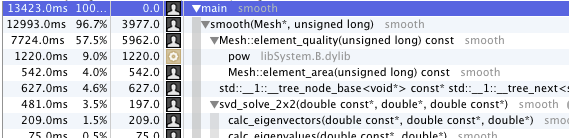
\includegraphics[scale=0.4]{profile.png}
\caption{Profiler output for intial run of Smooth}
\end{changemargin}
\end{figure}

As show in Figure \ref{fig:mem_util}, the program does not tax the memory system, given that the only updates are to two floating point values in the form of coordinate updates.
There are spikes in multiple CPU's as the process is moved onto different CPU's by the kernel. The profiler output for CPU utilisation is presented in Figure \ref{fig:cpu_util}
\begin{figure}[!h]
\begin{changemargin}{-20mm}{-20mm}
\center
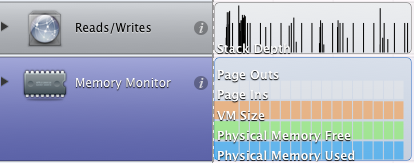
\includegraphics[scale=0.4]{mem_util.png}
\caption{Instruments output for RAM utilisation}
\end{changemargin}
\end{figure}

\begin{figure}[!h]
\begin{changemargin}{-20mm}{-20mm}
\center
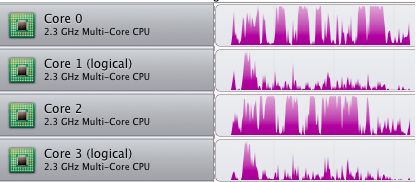
\includegraphics[scale=0.4]{cpu_util.png}
\caption{Instruments output for CPU utilisation}
\end{changemargin}
\end{figure}

\section{Optimising the serial implementation}
The \verb+Mesh+ class uses \verb+std::vector+ objects to encapsulate relationships between Nodes and mesh Elements.
However, adjacent Nodes have coordinates and metric values in spatially disparate places.
However, we will tackle this challenge on the GPU by passing vectorisable arrays to the device.
We gained execution speedup by re-writing the \verb+pow(f * (2.0 - f), 3.0)+ call explicitly as 3 multiplications:
\begin{lstlisting}[ ]
double F = f * (2.0 - f);
F = F * F * F;
\end{lstlisting}
which showed a 4.7\% improvement (from 7.05 seconds to 6.72).
Next, the branching code for the variable \verb+f = min(l/3.0, 3.0/l)+ was modified to eliminate the costly division operation:
\begin{lstlisting}[ ]
f = l < 3.0 ? l / 3.0 : 3.0 / l;
\end{lstlisting}
We also considered few purely mathematical (rather than architectural) optimisations.
Specifically, a call to \verb+smooth+ computes the 2x2 linear system:
\[
\mathbf{A}\vec{q} = \vec{p}
\]
by calling \verb+svd_solve_2x2+ $n \cdot m$ times, which uses singular value decomposition (SVD) to arrive at the solution.
A brute-force calculation showed another 5\% speedup.
Another mathematical optimisation relies on the observation that the code is attempting to converge on a smoother grid, while iterating through the nodes a fixed (200) number of times.
Empirically, we noticed that convergence was achieved after 10 such steps, thus making a 20-fold saving immediately.
For other grids, a more flexible approach can be used at no cost to measures the overall improvement in \emph{quality} in order to stop these iterations.
While the grids we studied exhibited quick convergence, there is no guarantee that this will be the case for other grids so we didn't include this as an optimisation.

We looked at speeding up the \verb+element_area+ function call.
Inside the \verb+element_quality+ function, the call to \verb+element_area+ retrieves the same data elements as its calling function.
However, combining them showed no effect, since the compiler already makes this optimisation in the code generation step.

\section{Parallelising using OpenCL}
For our first, naive, parallelisation attempt, we used OpenMP, a multicore programming framework, to distribute work among the CPU cores.
Although the loop controlling convergence of the algorithm could not be parallelised (since prior iterations had changed the mesh to an incrementally higher quality), the next loop, which iterated over the nodes, could be parallelised allowing us to utilise all available cores.
Although this saw a factor 2 speedup and produced almost identical results to the serial version, it returned non-deterministic output because of the data-conflicts when executing adjacent nodes by parallel threads of execution, leaving a lower quality grid than previously found.
When we inserted critical regions around every node's neighbours to stop data-conflicts, we saw a significant decrease in performance as threads stalled waiting for other threads to release their data locks.

To properly take advantage of OpenCL and the NVIDIA GPU on our testing platform, we chose to parallelise the work being done by the \verb+smooth+ function, which computes a \emph{quality} measure at each node, calculates updated coordinates for that node, then recomputes \emph{quality} to ensure that it improved.
It rolls back the changes results if \emph{quality} decreases.
The challenge of parallelising this code is twofold: eliminate contention between threads doing work on adjacent nodes, then write code to copy the relevant data to the GPU and do the correct computation within each thread.

\subsection{Mesh Colouring}
We employed a simple approach to ``colour'' the nodes, i.e. assign different values to non-adjacent nodes.
Colouring the nodes is necessary to ensure that concurrently executing threads on the GPU do not move coordinates of each other's adjacent nodes.
Our algorithm iterates over the nodes and assigns to itself the lowest unused colour among that node's adjacency list.
\begin{algorithm}[H]
\caption{Graph Colouring}
\label{al:colour}
\begin{algorithmic}[1]
\STATE Initialise colours[vid] to -1 $\forall$ vid
\FOR{$vid=1\hdots m$}
  \STATE colour = 0
  \FOR{$j=1\hdots n_{vid}$}
    \IF{colours[j] == colour}
      \STATE foundColour = false
      \STATE break
    \ENDIF
  \ENDFOR
  \STATE colours[vid] = colour;
\ENDFOR
\end{algorithmic}
\end{algorithm}
On the small mesh we studied, this algorithm used 7 colors to cover the mesh.  These 7 colors represent 7 iterations over which the GPU will make updates to the mesh, as each of those computations will be guaranteed to be free of contention.  

\subsection{OpenCL-specific Implementation}
OpenCL is a GPU computing framework supported by the open source community supported by most commercial GPU and CPU hardware.
Our code, to be executed on the device, is written in a \verb+Mesh.cl+ file.
The C++ program compiles this file and launches execution.  The outline looks as follows:
\begin{algorithm}[H]
\caption{OpenCL Program}
\label{al:colour}
\begin{algorithmic}[1]
\STATE 1) Compile Mesh.cl from Mesh.cpp
\STATE 2) Upload relevant data to the GPU
\STATE 3) run \verb+smooth+ kernel on the GPU
\STATE 4) download Mesh coordinates back to the CPU
\STATE 5) report results
\end{algorithmic}
\end{algorithm}
As OpenCL 1.1 does not support the Standard Template Library, we rewrote the data items as \verb+double+ and \verb+int+ arrays.  C++ style functions found in the \verb+Mesh+ class were rewritten for the GPU kernel.  As an example:
\begin{lstlisting}[ ]
bool isSurfaceNode(size_t vid);
void smooth(Mesh *mesh, size_t niter);
double element_quality(size_t eid);
\end{lstlisting}

became

\begin{lstlisting}[ ]
bool isSurfaceNode(size_t vid, __global uint *NEListOffs, __global uint *NNListOffs);
__kernel void smooth
(__global uint *NEList, __global uint *NNList,  __global uint *NEListOffs, __global uint *NNListOffs,
__global uint *ENList, __global double *metric, __global double *coords, __global double *normals,
__global uint *colorIdxs, const uint orientation, const uint NNodes, const uint colorOffset);
double element_quality(size_t eid, __global uint *ENList, __global double *metric, __global double *coords, int orientation);
\end{lstlisting}
These items are stored in the global memory of the GPU.  A further optimisation would be to move this data further into shared memory of each GPU warp, but nodes located near each other on the grid may be located in disparate places within the array.  The performance impact of this approach is questionable, but deserves further study.

After measuring benchmark results, we made further optimisations by exploiting vectorisation of data the GPU.  Here is the header file for this optimisation:
\begin{lstlisting}[ ]
__kernel void smooth
(__global uint3 *NEList, __global uint3 NNList,  __global uint *NEListOffs, __global uint *NNListOffs,
__global uint3 *ENList, __global double3 *metric, __global float2 *coords, __global float2 *normals,
__global uint *colorIdxs, const uint orientation, const uint NNodes, const uint colorOffset);
\end{lstlisting}
The data is accessed with greater bandwidth, but because NVIDIA writes data serially, we only saw a small performance increase.  Decreasing precision, while technically changing the problem being solved, helped with data throughput and did yield performance gains.

Further modifications to the original \verb+smooth+ kernel were also made.  We cached previously computed \verb+element_quality+ values for nodes which were not changed.  Thus these computations were not re-done.  Lastly, we looked at not calculating \emph{quality} when coordinates were unchanged.  However, since most of the time these coordinates were moved (by at least a small amount), this had a negligible effect.

\section{Results}
%  various charts and tables of data from running the code

% need to create a sample output for 5 runs of initial code
% need to create a sample output for 5 runs of final code

% need to produce a table with the following average times (3 grid sizes)
% initial code
% changing pow
% changing branch "l < 3.0..."
% changing matrix solver
% changing vector<> to double*
% naive OpenMP
% full OpenCL
% fullo OpenCL with vectorization

\section{Conclusion}
Mesh smoothing algorithms are an important step in the scientific computing pipeline.  Serial algorithms in this field  should pay special attention to how and where compute resources are spent.  Small, incremental improvements in instruction count or memory accesses in some function calls could have large implications for performance if those function calls represent a large percentage of overall compute time.  One should also balance these considerations agains the optimisations built into the compiler.  As we demonstrated, some attempts at increasing performance were met with failure because the compiler we chose, gcc, already does a very good job at optimising generated code.  The overwhelming conclusion from our research and experimentation shows that parallelism inherent in a program's structure is best exploited using the architecture in current GPUs.  However, re-phrasing the problem in a way to expose the parallelism is sometimes non-obvious.  The implementation of graph coloring ensure that concurrent executions of incremental mesh improvements did not interfere to produce inferior results.  We believe that an improved graph coloring algorithm could further reduce execution time as much as 20\%.

% reordering the nodes to keep all threads working, means eliminiating spacial locality didn't work


\end{document}
